\documentclass[11pt,a4paper]{article}

% french presentation rules
\usepackage[french]{babel}

% allow accents without commands
\usepackage[utf8]{inputenc}
\usepackage[T1]{fontenc}

\usepackage{url}
\usepackage{graphicx}

\begin{document}

\title{HLIN302~--- Projet « 1010! le casse brique »}
\author{Youcef Cherfaoui
	\and{Colin Geniet}
	\and{Victor Huesca}
	\and{Alexandre Ribeyre}}
\date{Janvier 2017}
\maketitle

\begin{abstract}
Ce projet vise à la création d'un clone sur terminal Unix du jeu pour mobile 1010!. Nous discutons dans ce rapport les choix faits et les méthodes utilisées durant la réalisation du projet.
\end{abstract}

\tableofcontents
\clearpage


\section*{Introduction}
\subsection*{Présentation du jeu}
Le jeu 1010!\footnote{\url{https://www.1010ga.me/}} est un jeu pour mobile de type puzzle disponible sur Android et iOS. Il consiste en une grille de taille $10\times10$~--- d'où le nom~--- où l'on place des pièces constituées de plusieurs carrés. Bien entendu, ces formes doivent être posées sur des espaces vides du plateau. Dès qu'une ligne ou une colonne est entièrement remplie, celle-ci est vidée.

\begin{figure}[h]
\centering
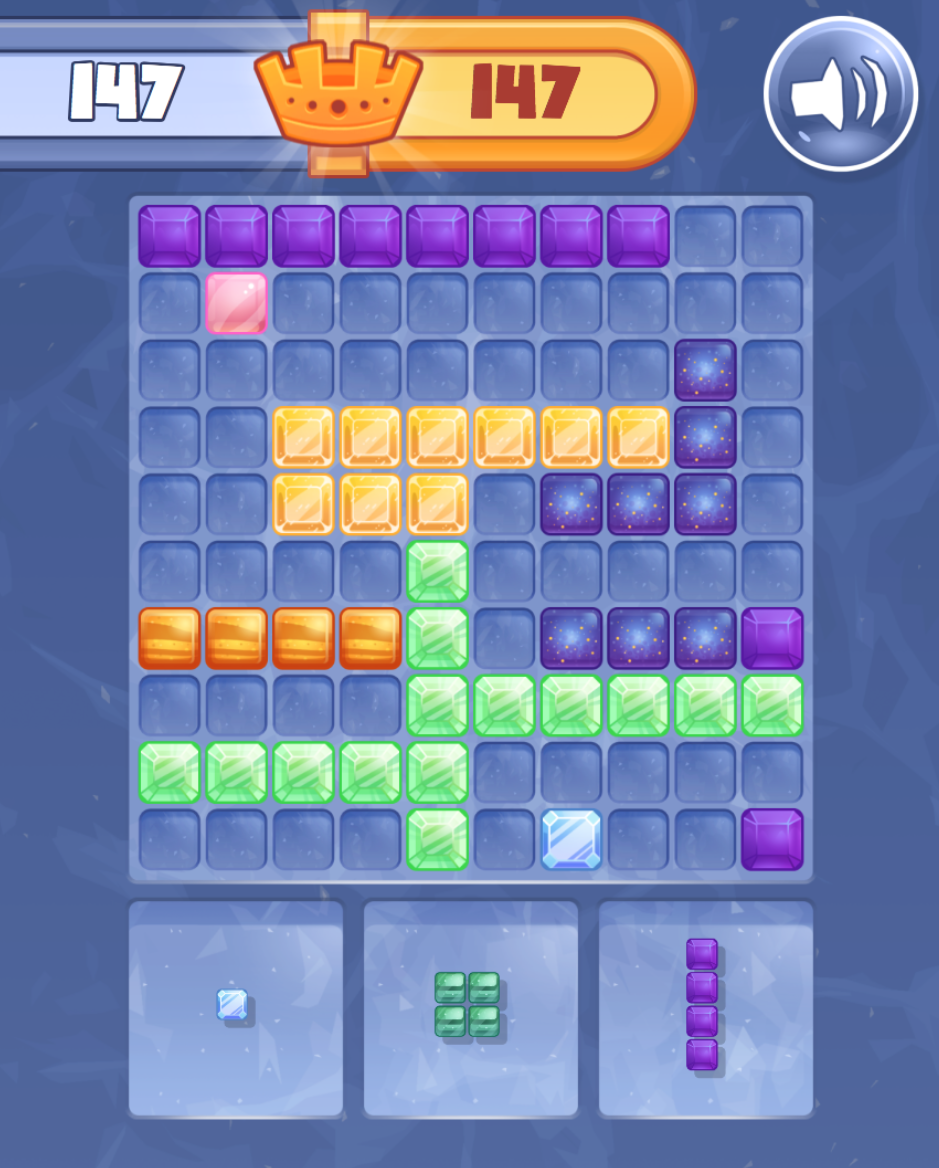
\includegraphics[width=0.5\textwidth]{image/1010_exemple.png}
\end{figure}

Les formes sont choisies aléatoirement dans un ensemble prédéfini et sont proposées trois par trois, c'est à dire que les trois nouvelles formes ne sont données que lorsque les trois précédentes ont été placées. Le jeu se termine dès qu'aucune des pièces disponibles ne peut être placée.

Le but est d'obtenir un score maximal. Celui-ci augmente en plaçant des formes (du nombre de carrés la formant) ainsi qu'en vidant des lignes et des colonnes (10 pour une ligne ou une colonne, avec des bonus lorsque plusieurs sont supprimées simultanément).

\subsection*{Le projet}
Le but de ce projet est donc de créer un clone de 1010! pour terminal Unix. Celui-ci devra donc être capable de reproduire exactement les règles du jeu original. Nous chercherons de plus à autoriser des variations sur celles-ci, telles que modifier l'ensemble des formes, leur probabilité d'apparition, et même les dimensions du plateau. Le jeu comprendra également un menu, un système de sauvegarde et un historique des mouvements permettant de les annuler.

D'un point de vue technique, selon les spécifications imposées, le jeu sera codé en C++ en utilisant pour l'interface la librairie ncurses\footnote{\url{https://www.gnu.org/software/ncurses/}}, spécifiquement prévue pour les interfaces graphiques sur terminal et disponible sur la plupart des systèmes Unix actuels (GNU/Linux, OpenBSD, FreeBSD\dots) ainsi que OSX.


\clearpage
\section{Moteur du jeu}
Le moteur est le cœur du jeu à proprement parler, par opposition à l'interface. Il comprend donc les structures permettant de décrire l'état du jeu, ainsi que les fonctions permettant d'effectuer toutes les actions du jeu.

\subsection{Représentation}
Trois classes sont utilisées pour représenter l'état des différents éléments du jeu :

\paragraph{Les formes} (classe \verb"Form")
Celles-ci sont représentées par un tableau de paires de coordonnées, chaque paire correspondant à un carré constituant la forme. Seuls les carrés `pleins' sont donc représentés. 

Le principal inconvénient de cette représentation est qu'elle est pas optimale pour l'ajout de nouveaux carrés dans une forme puisqu'elle nécessite de modifier la taille du tableau. Cependant, la taille des pièces est telle que ce problème est en pratique négligeable.

Une autre solution aurait été de les représenter par une grille (tableau bidimensionnel) de booléens : vide / plein. Cependant, cette méthode est plus complexe si la taille des formes n'est pas connue à leur création. Puisque nous nous sommes efforcés de ne pas contraindre le jeu aux dimensions du jeu original, la première solution a été retenue.

Afin de simplifier plusieurs opérations, la classe \verb"Form" calcule également les limites de la forme, c'est-à-dire le plus petit rectangle la contenant entièrement. Cela permet par exemple de déterminer immédiatement si une forme dépasse du plateau.

\paragraph{Le plateau} (classe \verb"Board")
Contrairement aux formes, sa représentation s'impose : c'est un tableau bidimensionnel représentant toutes les cases du plateau, chaque case étant représentée par un entier définissant sa couleur (ou bien 0 si elle est vide).

On notera que l'on ne peut pas décrire l'état du plateau par l'ensemble de formes qui y ont été placées, puisque la suppression des lignes et colonnes ne conserve pas ces formes. Il est donc nécessaire de décrire l'état de toutes les cases.

\paragraph{Le jeu} 
Pour finir, la classe \verb"mainGame" représente l'état du jeu dans son ensemble, en utilisant les deux classes précédentes :

\begin{itemize}
\item L'état du plateau est défini par une instance de la classe \verb"Board"
\item L'ensemble des formes est stocké dans un tableau (la possibilité d'accès aléatoire est importante), avec une couleur associée, et un poids influençant leur probabilité d'être sélectionnées aléatoirement. Les différentes informations sont regroupées dans une structure.
\item Les formes sélectionnées, c'est-à-dire les trois pièces à placer, sont indiquées par leurs indices dans l'ensemble des formes. Elles constituent un deuxième tableau. Dans le cas où la forme a été utilisée est n'a pas été remplacée, l'indice $-1$ indique l'absence de forme sélectionnée.
\end{itemize}

\subsection{Manipulation}
Les classes \verb"Form" et \verb"Board" ont essentiellement un rôle de structure de données. Par conséquent, leurs méthodes restent basiques et sont pour la plupart des accesseurs. Nous mentionnerons simplement deux méthodes de \verb"Board" permettant des interactions simples avec \verb"Form" : 
\begin{itemize}
\item \verb"addForm()" permet d'écrire une forme sur le plateau à des coordonnées données.
\item \verb"formCollide()" teste si une forme, à une position donnée, serait en collision sur le plateau.
\end{itemize}

\medskip
La classe \verb"mainGame", est en revanche, comme son nom l'indique, la classe principale du moteur, c'est-à-dire celle qui sera par la suite manipulée par le reste du programme. Par conséquent, ses méthodes permettent d'effectuer des actions complexes du jeu. Deux sont particulièrement importantes :
\begin{itemize}
\item \verb"add_form()" permet de tenter d'ajouter une des formes sélectionnées à une position donnée. Elle vérifie que le coup est valide, ajoute la forme au plateau le cas échéant et effectue toutes les actions nécessaires après le coup, à savoir nettoyer d'éventuelles lignes ou colonnes pleines, mettre a jour le score et sélectionner de nouvelles formes si les trois ont été placées.
\item \verb"move_available()" teste s'il existe un coup valide dans la configuration actuelle.
\end{itemize}

\medskip
Ces deux méthodes complexes constituent le centre du moteur. À l'interface près, on peut schématiser le jeu par la boucle
\begin{verbatim}
while(move_available()) {
    addform();
}
\end{verbatim}



\subsection{Fichiers de sauvegarde}
Le jeu intègre également un système permettant de sauvegarder et charger une partie dans un fichier. Celui-ci permet de sauvegarder les dimensions du jeu, l'ensemble des formes utilisées, l'état du plateau, les formes sélectionnées, ainsi que le score.

Ce même système sert également aux fichiers de configuration : on définit alors uniquement les dimensions et l'ensemble des formes, les autres éléments étant totalement optionnels.

Le choix d'utiliser un format unique pour la configuration et les sauvegardes est justifié par le fait que toutes les informations contenues dans un fichier de configuration sont également requises dans un fichier de sauvegarde : une sauvegarde ne définissant pas les règles~--- c'est-à-dire la configuration~--- est inutile.

Chaque classe du moteur contient donc des méthodes permettant de lire et écrire les informations qu'elle contient dans une chaîne de caractères. Ces méthodes sont ensuite utilisées par le menu pour permettre la lecture et l'écriture des fichiers de sauvegarde.


\section{Interface}
L'interface est la partie du programme qui permet à l'utilisateur d'interagir avec le jeu. Dans notre cas, elle a deux rôles majeurs : l'affichage et la gestion des contrôles. Comme mentionné précédemment, l'interface se fera via un terminal Unix, en utilisant la librairie ncurses.

\subsection{Organisation générale de l'interface}
Il existe deux parties principales de l'interface : le jeu à proprement parler et le menu. Celles-ci ayant relativement peu d'interactions, nous avons décidé de les séparer dans deux classes : \verb"gameWindow" et \verb"menuWindow". Il est toutefois nécessaire de relier ces deux dernières, ainsi que le moteur. Ceci est le rôle d'une troisième classe : \verb"mainWindow".

Le lien entre ces différentes classes est assuré par des pointeurs : \verb"mainWindow" a des pointeurs sur \verb"gameWindow", \verb"menuWindow" et \verb"mainGame". En retour, \verb"gameWindow" et \verb"menuWindow" ont un pointeur sur \verb"mainWindow". Le moteur pouvant fonctionner indépendamment de l'interface, \verb"mainGame" n'a en revanche pas de pointeur sur \verb"mainWindow". On notera enfin que les interactions entre \verb"gameWindow" et \verb"menuWindow" passent obligatoirement par \verb"mainWindow".

\begin{figure}[h]
\caption{lien entre les classes de l'interface graphique}

\centering
\setlength{\unitlength}{1mm}
\begin{picture}(115,50)
\setlength{\fboxrule}{1pt}
\put(5,5){\framebox(25,15)[t]{\parbox{25mm}{\center{jeu\\ \texttt{gameWindow}}}}}
\put(45,5){\framebox(25,15){\texttt{mainWindow}}}
\put(85,5){\framebox(25,15)[t]{\parbox{25mm}{\center{menu\\ \texttt{menuWindow}}}}}
\put(45,30){\framebox(25,15)[t]{\parbox{25mm}{\center{moteur\\ \texttt{mainGame}}}}}

% .2mm shorter for the frames
\put(57.5,20){\vector(0,1){9.8}}
\put(30, 11){\vector(1,0){14.8}}
\put(45, 14){\vector(-1,0){14.8}}
\put(70, 14){\vector(1,0){14.8}}
\put(85, 11){\vector(-1,0){14.8}}
\end{picture}
\end{figure}

En pratique, tous ces pointeurs sont initialisés lors de la construction de \verb"mainWindow", qui crée également les instances des autres classes. Dans la mesure où ces pointeurs sont nécessaires au bon fonctionnement de ces différentes classes, il n'est pas prévu que des instances de \verb"gameWindow" ou \verb"menuWindow" soient créées en dehors de la construction d'une instance de \verb"mainWindow". Cette dernière constitue par conséquent la classe principale du programme (i.e.\ celle qui sera créée dans le \verb"main()").


\subsection{Méthodes d'interface}
Afin de compléter cet ensemble de pointeurs, la classe \verb"mainWindow" définit des méthodes «d'interface» : des méthodes qui se contentent d'appeler la méthode correspondante dans une des sous-classes. Ces méthodes constituent une grande partie de la classe \verb"mainWindow". Appelées via les pointeurs reliant les classes, elles permettent les interactions entre les trois classes de l'interface graphique.

Quelques-unes d'entre elles méritent une attention supplémentaire :

\paragraph{Fenêtre active}
Un autre rôle de la classe \verb"mainWindow" est de gérer la fenêtre active (menu ou jeu). Le choix de celle-ci est représenté grâce à une énumération. Sa valeur a une influence sur deux méthodes : \verb"print()" (méthode principale d'affichage) et \verb"input()" (traitement des entrées du clavier). En effet, ces méthodes appelleront la même méthode dans la classe \verb"gameWindow" ou \verb"menuWindow" selon laquelle des deux est active.

\paragraph{Accesseur(s) du moteur en écriture}
L'accès en écriture au moteur du jeu par les classes de l'interface graphique pose un problème : puisque les dimensions du plateau ne sont pas imposées, il est possible que celles-ci changent. Cela nécessite alors de recréer les fenêtres d'affichage du jeu. La possibilité de changer ces dimensions est importante, mais il va de soi que l'on ne veut pas pour autant recréer les fenêtres dès qu'une action est effectuée sur le jeu.

La solution que nous avons choisie est de créer deux accesseurs en écriture :
\begin{itemize}
\item 
\verb"setgame()" est inconditionnel : il correspond à l'idée de changer de partie, et permet donc une modification des dimensions. Son appel recrée donc les fenêtres d'affichage, et il ne doit donc pas être trop utilisé.
\item
\verb"changegame()" correspond à une modification du jeu au cours d'une partie. Il interdit les modification des dimensions, et est de fait plus simple.
\end{itemize}

Cette distinction sémantique entre les deux accesseurs permet en outre d'intégrer des opérations d'initialisation dans \verb"setgame()" : par exemple, l'historique des coups y est vidé, puisque l'on ne veut pas le garder en changeant de partie.

\subsection{Signaux d'entrée}
Les signaux d'entrée du clavier sont gérés par les méthodes \verb"input()" des classes \verb"mainWindow", \verb"gameWindow" et \verb"menuWindow". Comme mentionné précédemment, c'est normalement la méthode de \verb"mainWindow" qui est appelée, et qui transmet simplement le signal à l'une des deux autres.

Ces méthodes prennent en paramètre un entier correspondant à un signal transmit par une des fonctions d'entrée de ncurses, telle que \verb"getch()". Un switch associe aux différents signaux les actions appropriées.

\subsubsection{Gestion de la souris}
Le même système sert à gérer la souris : si le terminal le permet, les actions de celle-ci sont indiquées par un code spécial reçu comme un signal venant du clavier. Après sa réception, ncurses permet de récupérer une structure contenant toutes les informations concernant la souris.

Il existe cependant un problème : le comportement standard d'un terminal supportant l'usage de la souris est de ne transmettre de tels signaux que lorsque l'état des boutons de la souris change. Dans ce cas, il est impossible de recevoir un simple mouvement de la souris. Cela la rend peu intéressante pour un jeu vidéo : on souhaite pouvoir déplacer une forme sur le plateau avec le curseur.

Sous Linux, avec des émulateurs de terminal dérivés de Xterm, nous avons pu résoudre ce problème en modifiant la variable d'environnement \verb"TERM" qui contrôle le comportement du terminal : en lui assignant la valeur \verb"xterm-1003", le terminal transmet tous les mouvements de la souris, permettant le comportement attendu.

Dans tous les cas, l'usage de la souris restant entièrement dépendant du terminal utilisé, nous avons choisi de le laisser désactivé par défaut, l'option \verb"--enable-mouse" permettant de le réactiver.

\subsection{Affichage}
Nous avons choisi de baser l'affichage du jeu sur des carrés de couleur. Ceux-ci sont constitués de deux caractères ``espace'', ce qui donne une forme proche d'un carré avec la plupart des polices. La couleur d'arrière-plan est modifiée pour changer celle du carré.

Pour simplifier l'affichage du jeu, plusieurs fenêtres de ncurses (i.e.\ l'objet \verb"WINDOW") sont utilisées pour les différents éléments de l'interface : une pour les scores, une pour le plateau et trois pour les formes à placer. Une dernière fenêtre sert d'arrière-plan : elle est vide, colorée uniformément. Les autres fenêtres sont affichées par dessus.

Pour permettre de changer les dimensions du jeu, la taille et la disposition de ces fenêtres sont calculées par la méthode \verb"init_windows()" lors de la création de la classe \verb"gameWindow", et à chaque fois que les dimensions sont modifiées.

L'utilisation de fenêtres multiples permet d'effectuer ces calculs de positionnement à la création des fenêtres uniquement, ce qui rend les méthodes d'affichage plus simples.


\subsection{Historique}
Le jeu intègre un historique, permettant d'annuler les coups jusqu'au début de la partie et bien sûr de les rétablir. Il est implémenté par la classe générique\verb"History" et est intégré dans la classe \verb"gameWindow".

En mémoire, il est implémenté comme une liste doublement chaînée. En effet, l'historique nécessite de pouvoir facilement ajouter des éléments, et le parcours se fait uniquement par incréments et décréments. Une liste doublement chaînée permet d'effectuer toutes ces opérations en temps constant.


\clearpage
\appendix

\section{Liste des fichiers}
\subsection*{Sources}
\begin{tabular}{lp{76mm}}
\verb"board.cpp/.h" & classe \verb"Board" \\
\verb"color.cpp/.h" & initialisation et gestion des paires de couleurs pour ncurses \\
\verb"config_load.cpp/.h" & fonctions utilisée pour la lecture des fichiers de configuration \\
\verb"form.cpp/.h" & classe \verb"Form" \\
\verb"game_window.cpp/.h" & classe \verb"gameWindow" \\
\verb"global_log.cpp/.h" & stream de sortie écrivant sur stderr et sur le fichier log.txt \\
\verb"history.tcc/.h" & classe générique pour l'historique \\
\verb"includeGUI.h" & inclut les classes \verb"mainWindow", \verb"gameWindow" et \verb"menuWindow". Celles-ci sont interdépendantes et nécessitent d'être incluses les trois ensemble, et dans un ordre particulier \\
\verb"main.cpp" & \verb"main()", initialisation de ncurses, initialisation du jeu et boucle principale \\
\verb"main_game.cpp/.h" & classe \verb"mainGame" \\
\verb"main_window.cpp/.h" & classe \verb"mainWindow" \\
\verb"menu_window.cpp/.h" & classe \verb"menuWindow" \\
\verb"option.cpp/.h" & gestion des options en ligne de commande \\
\end{tabular}

\subsection*{Sauvegardes~--- configuration}
\begin{tabular}{lp{84mm}}
\verb"default_board" & configuration par défaut (règles du jeu original) \\
\verb"exemple_board" & exemple de fichier de configuration, avec le détail de la syntaxe \\
\verb"standard_board" & règles demandées dans les spécifications \\
\verb"autosave" & fichier de sauvegarde automatique (sauvegarde en quittant le jeu) \\
\verb".highscore" & sauvegarde des scores \\
\end{tabular}

\end{document}